\section{Normalizing Flows}\label{sec:nf}
Normalizing Flows are an explicit density function that learns a tractable
density. To do this Flows use the change of variable methods to learn a
tractable density function that can be learned and use the change of variable
method~\ref{eq:cov} to map to the intractable density function. 

\begin{equation}
p(x) = q(f^{-1}(x))|det\frac{df^{-1}(x)}{dx}|
\label{eq:cov}
\end{equation}

The change of variable method works because the integral of all probability
density functions is 1 ($\int p(x)dx = \int q(z)dz = 1$). Through this
Flows are composed of a series of bijective functions, that is functions that
are one-to-one and onto another data space. This is shown in
Figure~\ref{fig:nf}.

\begin{figure}[ht]
\centering
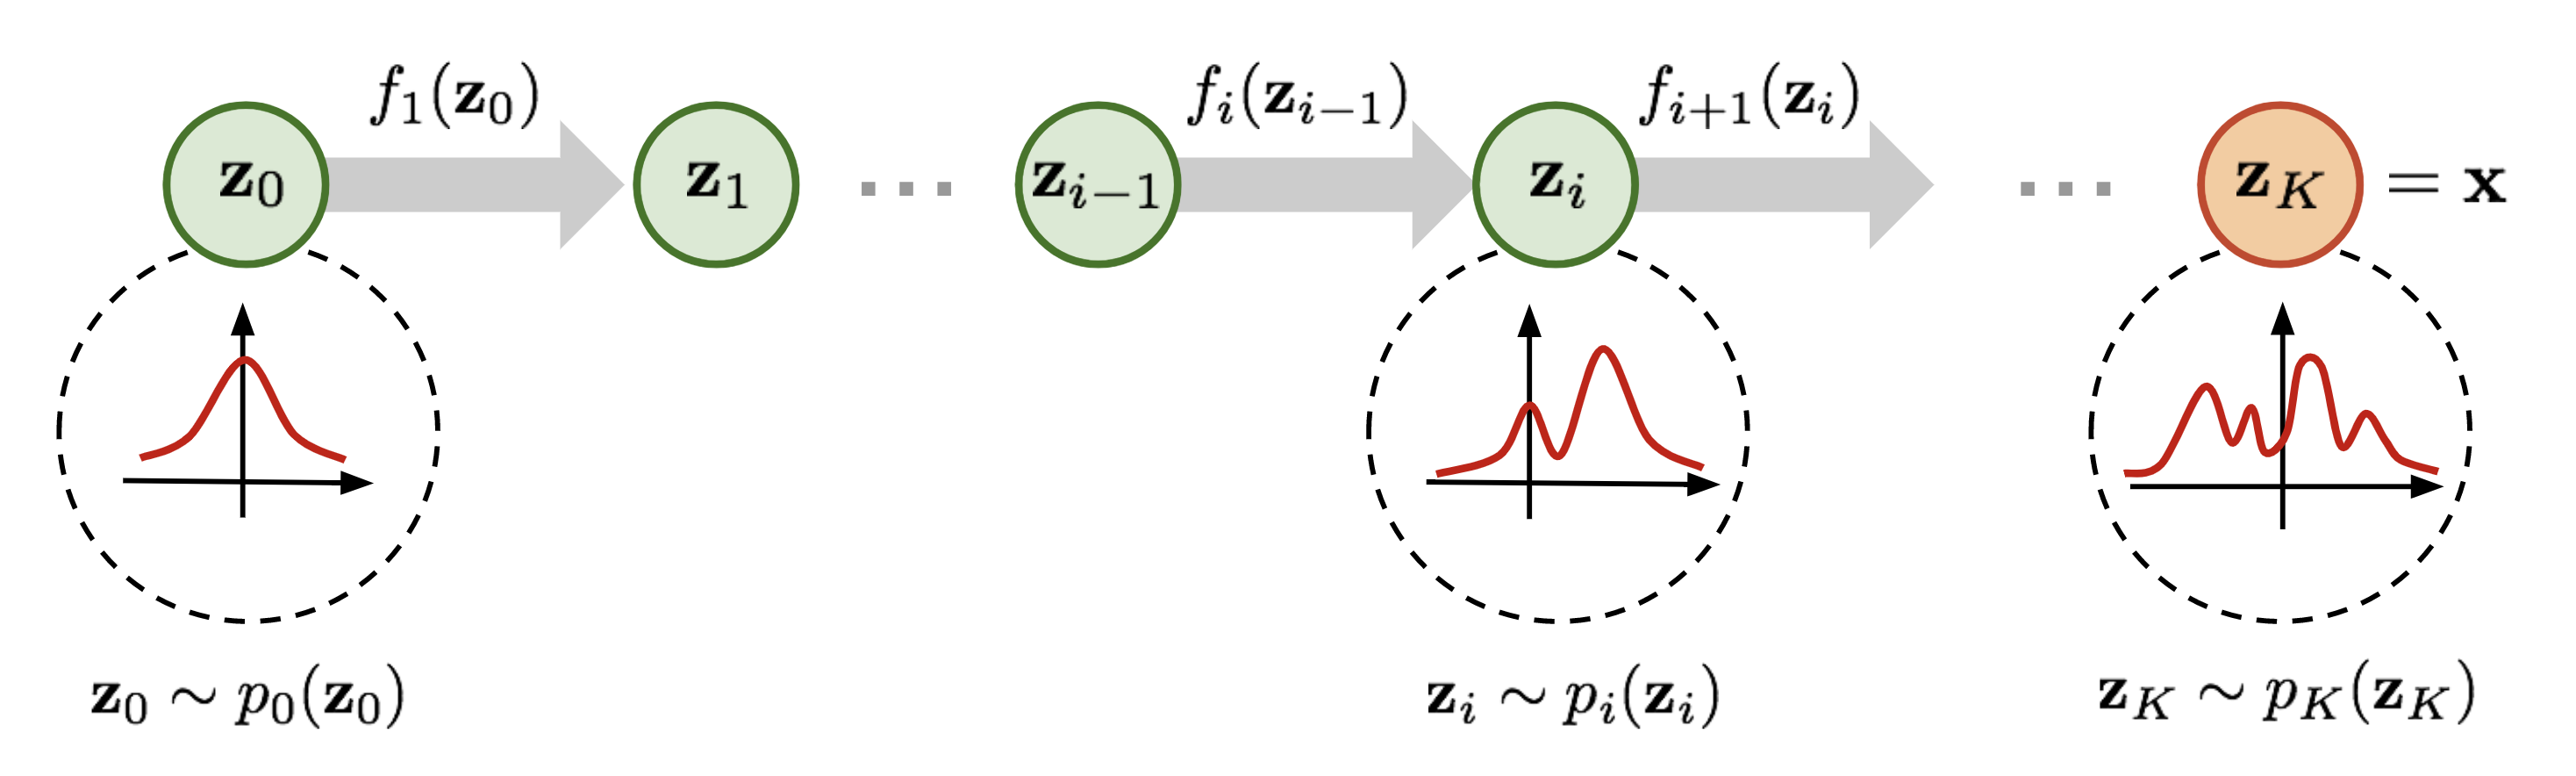
\includegraphics[width=0.48\textwidth]{normalizing-flow.png}
\caption{Architecture of a normalizing flow}
\label{fig:nf}
\end{figure}

Normalizing flows are bidirectional models, in that they are trained in both
directions. Because of the bijective nature of these networks one samples from
the tractable distribution and the input data and send them backwards through
the network. The loss function is then used to learn the difference between
these distributions. This makes flows unsupervised learners. 

\subsection{GLOW}
GLOW~\cite{GLOW} was the first normalizing flow that was able to generate realistic looking
images with larger datasets like CelebA. GLOW is based on two predecessors,
NICE~\cite{NICE} and RealNVP~\cite{RealNVP}, and essentially is a much larger version of
RealNVP with some minor changes. GLOW showed that like traditional deep neural
networks, normalizing flows could generate substantially better results by
deepening the network. The other major contribution that GLOW improves from
RealNVP is that GLOW uses a 1x1 invertible convolutional layer. The architecture
of GLOW is shown in Figure~\ref{fig:glow}.

\begin{figure}[ht]
\centering
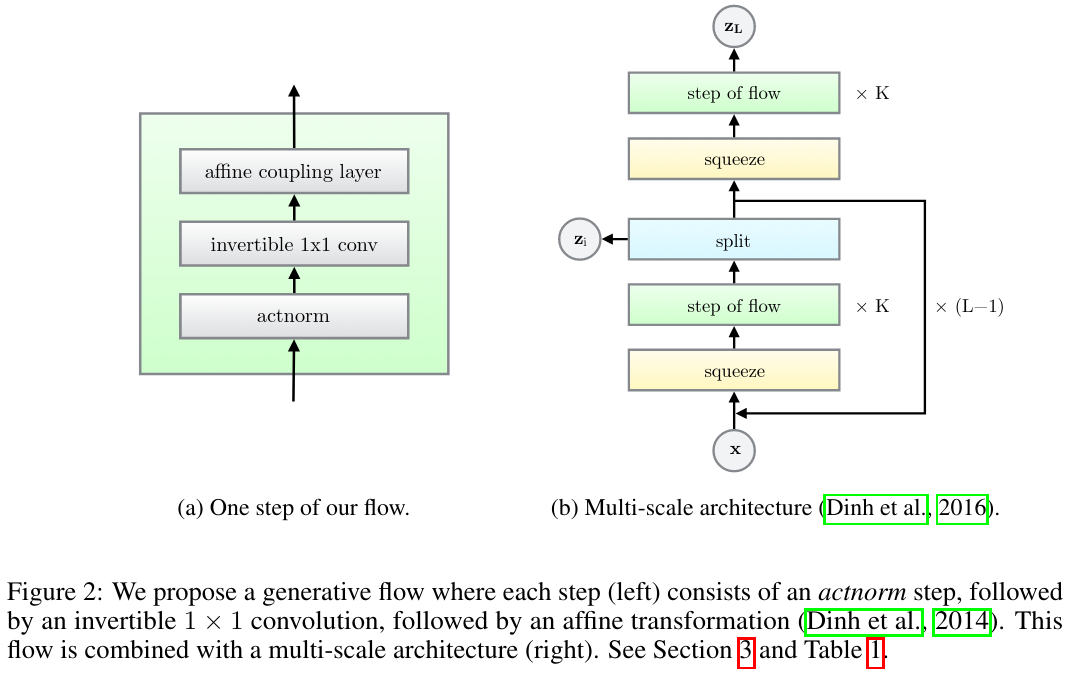
\includegraphics[width=0.48\textwidth]{GLOWModel.png}
\caption{Construction of GLOW}
\label{fig:glow}
\end{figure}

The key parts of this type of flow is that there is a multi-scale architecture
that is able to learn different scales of the data. This multi-scale
architecture allows the network to better learn fine detail in data and this
provides the higher resolution achieved by this network. The larger the data
being trained on, the more layers are needed for accurately reproducing data.
The major downside of flows is that they are substantially more difficult to
train than networks like VAEs or GANs. The advantage of these networks is that
they are able to learn the density, and thus it is trivial to infer between
different latent variables. For example, it is easy to introduce glasses on a
face by performing a linear interpolation between the image and the center of
images with glasses. The center of images with glasses can similarly be easily
found by taking the mean of several images that have glasses in them, requiring
one to know the feature that is being looked for.
